\chapter{Background}

\section{Scans}

\section{SIMD}

The idea behind SIMD (Single Instruction/Multiple Data) architectures as
firstly classified by Flynn \cite{flynnsimd}, is to use a single instructions
stream to process many different values at once. The earliest members of this
class of architectures were the vector processors of the 1970's such as the
Cray 1 or the Earth Simulator, fastest supercomputer in the world in the year
2002 \cite{hennessyarch}. In a vector processor the size of a register is not
static but the number of elements in a register can be configured at runtime up
to a certain limit, the Cray 1 had a limit of 64 values in a register, each of
the values 64 bits wide. When arithmetic instructions are executed with such a
vector register in its operand the individual values can be processed in parallel
as far as resources permit. So processing a 64-element vector can take
significant less than 64 cycles. Load operations typically gather values that
can be scattered throughout memory into a single registers and load operations
have to disperse the values back into memory. By this approach a vector
instruction set has dramatically fewer instructions than an architecture that
operates on a single value at a time. This frees up instruction decoding
resources that can be repurposed to increase throughput elsewhere.

However, classic vector architectures have not become the most prevalent model
for modern processor architectures, obvious reasons being:
\begin{itemize}
\item Superscalar out-of-order processors already provide parallelism by
automatically identifying independent instructions and executing them
simultaneously.
\item Gathering loads and scattering stores are not a good fit for caches and
memory organized in fixed-size blocks where at least a full block is fetched or
stored. This would waste a significant amount of memory bandwidth and cache
memory.
\item The large variable-length registers add additional state to the processor.
\end{itemize}

In the end a fairly limited subset of a vector architecture has found its way
into virtually any instruction set but the most reduced for embedded
applications. These so called multimedia instructions only support a fixed-size
registers which can usually be overlaid with different data types, for example
registers containing 128 bits can be used as either four 32-bit values or eight
16 bit values. This means there are many different instructions compared to the
approach taken by vector architectures. Scattering and gathering is usually not
present or only in a limited form by loading values separated by a constant gap.
Examples for this form of vector instructions are MMX, SSE and AVX on Intel
CPUs, AltiVec on PowerPC or NEON on ARM processors.

To understand why SIMD still provides an advantage over superscalar
instruction-level parallelism the latency and throughput of normal instructions
has to be taken into account. In table~\ref{tab:latencies} the latencies and
throughput for loads and additions are shown. Now imagine a loop creating a sum
over 32-bit values; requiring a load and an add. All instructions are fully
pipelined so we can load two 32 bit integers and perform two additions per
cycle, the full throughput is not achievable because we cannot load more than
two values. Now we change the loop to work on 256 bit vectors, the load
throughput does not change with size so we can load 16 32-bit integers per cycle
and still perform 2 full adds, adding all 16 integers. In theory we now
increased the throughput eightfold. In practice the performance will be bound be
bound by memory latency in this simple example though, unless the number of
arithmetic instructions is increased.

\begin{table}\center
\begin{tabular}{c|c|c}
Instruction & Latency & Throughput\\
\hline
Scalar load & (depends on cache) & 2 per cycle\\
Scalar add & 1 cycle & 4 per cycle\\
%Scalar mul & 3 cycles & 1 per cycle\\
Vector load & (depends on cache) & 2 per cycle\\
Vector add & 1 cycle & 2 per cycle\\
%Vector mul & 5 cycles & 1 per cycle
\end{tabular}
\caption{Instruction latencies and throughput on Intel Haswell}
\label{tab:latencies}
\end{table}

\section{SIMD on Modern Hardware}

The focus of this section lies on the current 4th generation Intel Core
architecture. The basic observations are also applicable to any other current
architecture or SIMD instruction set, but the performance characteristics may
differ widely.

Intel has a long history supplying multimedia instruction sets:
\begin{description}
\item[MMX] The Multi Media eXtension made the start in 1997, supplying integer
instructions on 64 bit registers shared with the existing floating point unit.
\item[SSE] The Streaming SIMD Extension added a fully independent 128 bit
register set in 1999. SSE only supported floating point operations, SSE~2 added
the integer counterparts in 2001. SSE was extended with many different
instructions often catered towards operations commonly found in video codecs.
\item[AVX] The Advanced Vector eXtensions extend the registers introduced in
SSE to 256 bits. As with SSE, AVX provided only floating point operations and
AVX~2 added integer instructions. AVX also provides new encodings for all
existing SSE instructions using a three-operand form instead of the more
restricted two-operand form used by SSE. AVX instructions generally behave as
if working on two independent 128 bit registers instead of one large 256 bit
register, this makes operations that combine bits from the lower 128 bits with
bits from the upper 128 bits of the register more complex.
\item[AVX-512] AVX 512 is a new instruction set extending the AVX registers to
512 bits. While it contains interesting new operations that could be very
useful for implementing scans it was not available in general purpose CPUs at
the time this thesis was written.
\end{description}

Since AVX~2 is currently the latest available set of SIMD instructions on Intel
hardware it will be the focus of this thesis. It provides 16 256-bit registers
and integer operations on 32 8-bit, 16 16-bit, 8 32-bit or 4 64-bit values at a
time.

As a preliminary it is vital to understand how caches are organized on a
current Intel CPU. Since for a scan data will almost always be loaded freshly
from DRAM cache levels are ignored here. The cache on any recent Intel CPU is
partitioned into cache lines of 64 bytes. This means that when reading data
from memory it does not matter if 1 byte or 32 bytes, which is the maximum load
size in AVX~2, are read at a time and the whole cache line will be fetched from
DRAM.

A scan over an array of integers of size 8, 16, 32 or 64 bits can be
easily implemented in SSE or AVX as illustrated in
figure~\ref{fig:simplecomparesse}. Here a greater than predicate is executed,
the \texttt{pcmpgt} instruction takes two vectors and sets the corresponding
element in a result vector to either all ones if the element in the first
vector is greater than the element in the second vector. Otherwise it is set to
zero. To generate a bit vector from this result the \texttt{movmsk} instruction
is used which takes the most significant bit of every element in a vector and
sets the bit with the same number in a simple integer. In the example the
result of \texttt{movmsk} is $00111101$ in binary or $3d$ in hexadecimal.

\begin{figure}\center
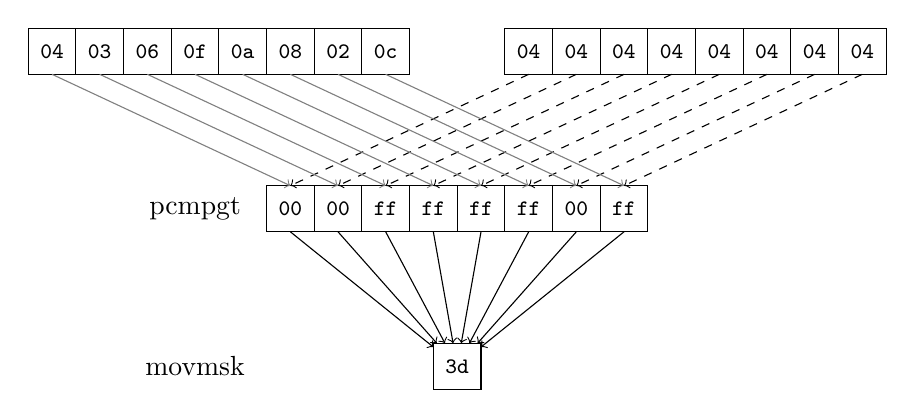
\begin{tikzpicture}[node distance=2cm]

\def\elemwidth{4ex};
\def\dotswidth{4ex};
\def\labelsepa{0.2cm};
\tikzset{simd element/.style={
    rectangle,
    draw,
    inner xsep=0.1ex,
    font=\footnotesize\ttfamily,
    minimum width=\elemwidth,
    minimum height=1.666em
}};

\foreach \val [count=\i] in {04, 03, 06, 0f, 0a, 08, 02, 0c} {
    \node[simd element] (src1\i) [
        xshift=(\i-1)*\elemwidth, outer sep=0] {\val};
}

\foreach \val [count=\i] in {04, 04, 04, 04, 04, 04, 04, 04} {
    \node[simd element] (src2\i) [
        xshift=(10+\i-1)*\elemwidth, outer sep=0] {\val};
}

\foreach \val [count=\i] in {00, 00, ff, ff, ff, ff, 00, ff} {
    \node[simd element, below of=src16] (src3\i) [
        xshift=(\i-1)*\elemwidth, outer sep=0] {\val};
}

\node[label, below of=src14] (pcmp) {pcmpgt};

\foreach \i in {1,...,8} {
    \path[->, color=gray] (src1\i.south) edge (src3\i.north);
    \path[->, dashed] (src2\i.south) edge (src3\i.north);
}

\node[simd element, below of=src34] (src4) [xshift=\elemwidth/2, outer sep=0] {3d};

\foreach \i in {1,...,8} {
    \path[->] (src3\i.south) edge (src4);
}

\node[label, below of=pcmp] (movmsk) {movmsk};
\end{tikzpicture}
\caption{Comparing two vectors and generating a bit vector in SSE}
\label{fig:simplecomparesse}
\end{figure}

\section{\simdscan{}}

\simdscan{} \cite{SIMD-Scan} takes the basic idea shown in
figure~\ref{fig:simplecomparesse} and extends it to arbitrary bit widths.
